\documentclass[12pt,a4paper]{article}
\usepackage[latin1]{inputenc}
\usepackage{amsmath}
\usepackage{amsfonts}
\usepackage{amssymb}
\usepackage{graphicx}



\begin{document}
\begin{titlepage}
   \begin{center}
       \vspace*{1cm}
 
       \textbf{{\huge Verslag Roadfighter}}
 
       \vspace{0.5cm}
        Project gevorderd programmeren
 
       \vspace{1.5cm}
 
       \textbf{{\Large Stijn Rosaer}\\20172195}
  
       \vspace{10cm}
 
       
\includegraphics[scale=0.4]{img/logoua.jpg}

       Januari 2019
 
   \end{center}
\end{titlepage}
\newpage

\section{Game}
De game bestaat uit een klasse \"Game\" die alles zal controleren en in een goede volgorde gaan aanroepen. Dit vormt dus een centrale plaats om controles uit te voeren op de toestand van het spel waardoor ik besloten heb om hier de distance, score, background, factory, world, \ldots bij te houden.\\
De world bezit alle objecten die tijdens het spel voorkomen. Deze komen daar door middel van abstract factoring die de objecten terug geeft als een shared entity pointer. Wanneer een object verwijderd moet worden, zal dit ook van hieruit gebeuren.\\
Een update van alle elementen gebeurt eveneens vanuit world. Door composition design pater zal ik van hieruit voor elke bijgehoude entity de update aanroepen, idem. voor draw.\\
\linebreak
Om het spel "speelbaar" te maken en een constante snelehid te hebben over alle computers start in in het begin van elke loop over mijn spel een timer, op het einde wacht ik dan de tijd die nog resteerd om een frame rate te bekomen van 30 fps..\\
Het genereren van passing cars gebeurt random op een locatie bepaald met mijn Random singleton. Wanneer er een gegenereerd wordt is afhankelijk van een functie die ik uit voer nl. wanneer je verder zit in het spel, zullen er meer auto's komen, als je trager rijd zullen er minder frequent gegenereerd worden om zo een evenwicht te bekomen.\\
\linebreak
Door het gebruik van observer patern kan ik doorgeven vanuit mijn observables (PlayerCar, Bullet en PassingPointsCar) wordt mijn observer (Game) aangeroepen die ervoor zorgt dat telkens de juiste actie onderno

\section{Objects}
Elk object bezit de nodige eigenschappen op de meest voor de hand liggende plaats in de minst afgeleide klasse. Zo bevind zich de stuct boundries zich in entity welke een top left, botom right, center, width en height bevat om zo gemakkelijk door te kunnen geven. Voor het controleren van collisions heb ik er voor gekozen om deze functie te implementeren in Entity omdat het me logisch leek omdat een entity botst. Hiervoor geef ik een vector mee van entities omdat ik dan zelf kan kiezen welke botsingen effectief effect hebben.
\newpage
Elk object wordt volledig vanuit de logische kant gecontroleerd. Dit betekened dat beslissingen en bewegingen van hieruit gestuurd worden en dat de grpahische kant enkel voor het displayen is. In de grafische kant zal dus ook de transformation singleton gebruikt worden om deze omzetting te doen.

\section{Background \& movenment}
Om een perceptie van snelheid te creeren heb ik de achtergrond als een lus door laten lopen aan de snelheid van de speler. Elk ander object krijgt zelf een snelheid en in de update functie zal de snelheid van de speler mee door gegeven worden waaruit de relatieve snelheid wordt berekende en hoeveel het object dus relatief moet verplaatsen.

\section{Racing car \& special passing car}


\section{Interaction}
Hieronder is een overzicht te vinden van de inheritace tussen de voornaamste klassen. Extra schemas's en documentatie zijn te vinden in de DOC folder gegenereerd door doxygen.\\
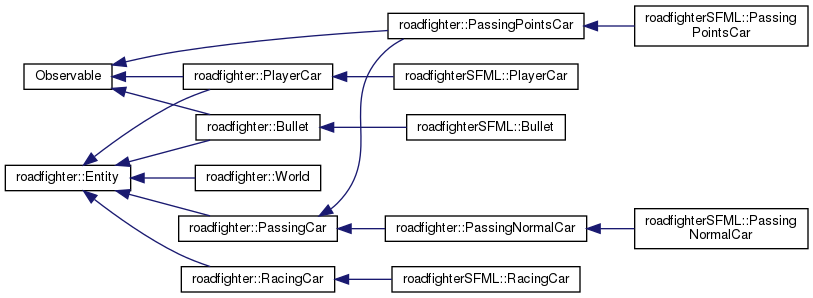
\includegraphics[scale=0.5]{img/inherit_graph_2.png}
\end{document}